\section{Soft and Collinear divergences in QED}

We're about to begin out last topic! It's slightly advanced - it's dealing with the fact that $S$-matrix cannot be formally defined in a theory without a mass gap. This technique is crucial if you continue on in particle physics, physics of jets, colliders etc. In QED, the photon is a massless particle, causing the problem; the precise issue is that single particle states cannot be distinguished from the multi-particle continuum; few particle ``out'' states look the same as few particle ``out'' states + soft/low-energy photons.

\subsection{Sketching the problem}

The dispersion if we only had electron looks like:

\begin{center}
    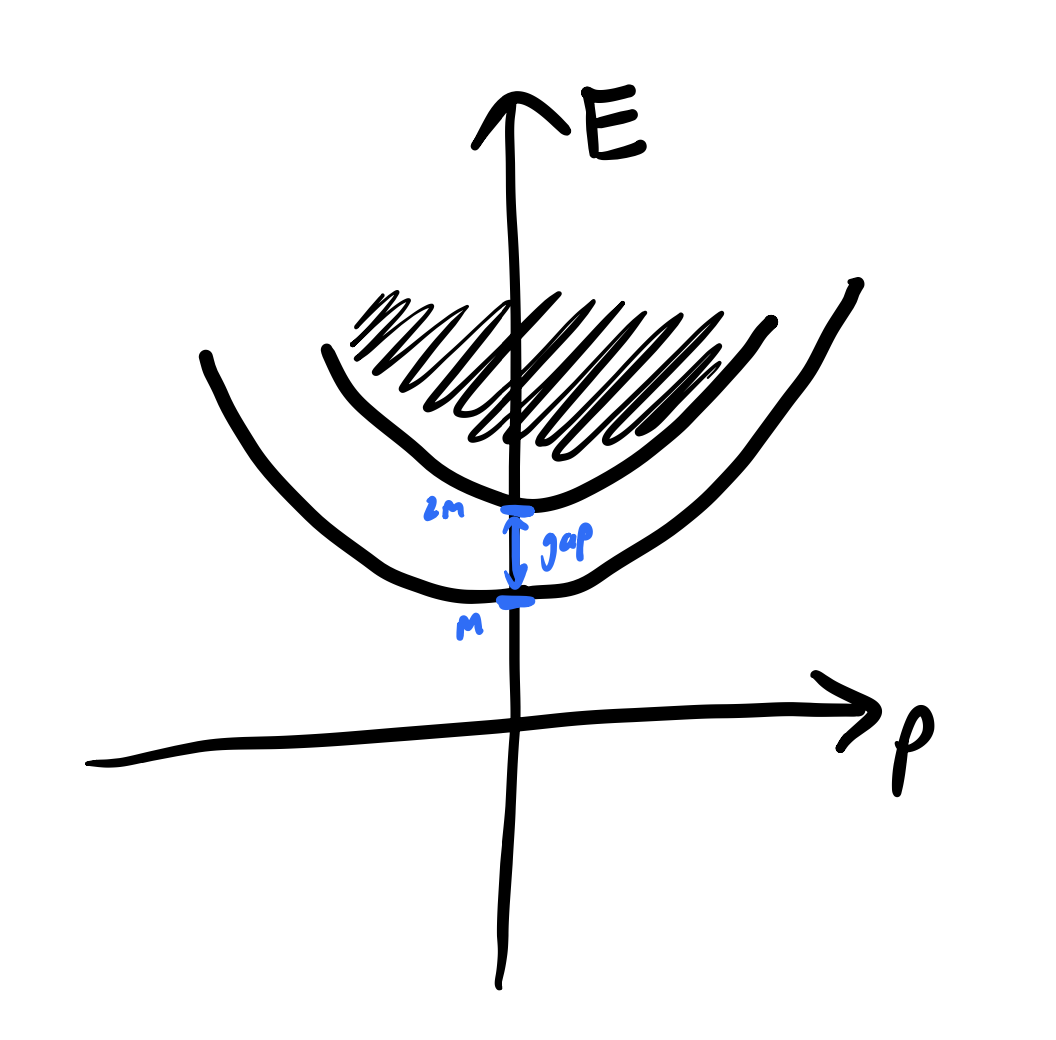
\includegraphics[scale=0.35]{Lectures/Images/lec14-massgap.png}
\end{center}

i.e. the theory has a gap, allowing us to define the $S$-matrix. But in QED, we now have photons, so we have a continuum of electron + photon states:

\begin{center}
    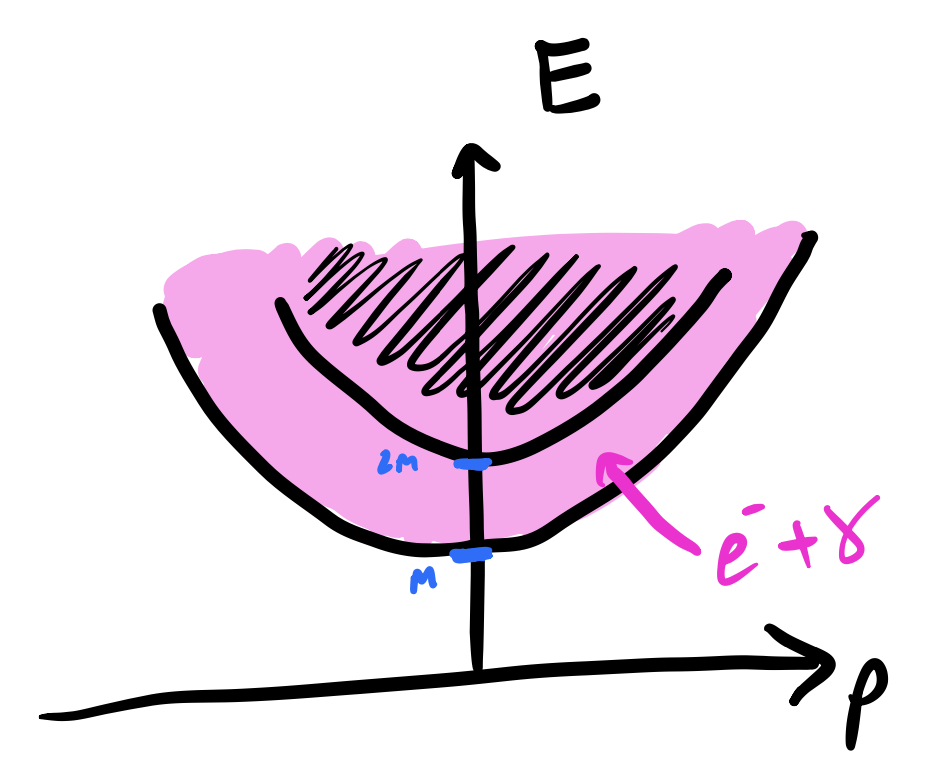
\includegraphics[scale=0.35]{Lectures/Images/lec14-nogap.png}
\end{center}

In equations, an $e^-$ at momentum $\v{p}$ has energy:
\begin{equation}
    E = \sqrt{\v{p}^2 + m^2}
\end{equation}

And a $e^- + \gamma$ state at total momentum $\v{p}$ has $e^-$ with momentum $\v{p} - \v{k}$ and $\gamma$ with momentum $\v{k}$, so the energy is:
\begin{equation}
    E = \sqrt{(\v{p}-\v{k})^2 + m^2} + \abs{\v{k}} = \sqrt{\v{p}^2 + m^2} + \mathcal{O}(\abs{\v{k}})
\end{equation}
and crucially, there is no gap because $\v{k} \to 0$ continuously in infinite volume. For finite size, $k = \frac{2\pi}{L}$ becomes quantized; this is a hint for the resolution.

One cannot ignore this issue; loop corrections to matrix elements will have IR divergences, also known as ``soft'' divergences. These are divergences of a very different type as UV divergences we have seen prior. Either we have an EFT which the UV divergence indicates that there is a scale which the theory breaks down, or the theory is UV-complete in which the case that the divergences can be regulated/removed by counterterms.

What does the IR divergence tell us about the theory? It doesn't tell us that the theory has a problem (indeed we found that QED is IR-free from our RG analysis)! Rather, it tells us that the observables we are choosing are bad. Here, we will see that the divergences arise in the step of putting the external particles/legs on shell in LSZ. The ``off-shell'' correlators that we have been studying (e.g. $\avg{\mathcal{T}\ldots}_c$) that we have been studying are always well-defined; it is only when we take specific limits (in order to put external legs on shell) that problems arise. 

These will get resolved if we accept the fact that we cannot distinguish $\ket{\psi}$ of interest with $\ket{\psi + \text{soft photons}}$. Fortunately, we will not have to consider an arbitrary number of soft photons. For example at 1-loop order the cross-section $\sigma$ is finite if we include states with one extra soft photon. Diagramatically:

\begin{center}
    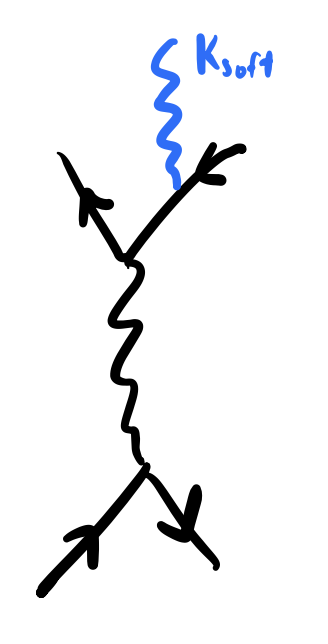
\includegraphics[scale=0.35]{Lectures/Images/lec14-singlesoft.png}
\end{center}

Specifically, we will see that the cross-section:
\begin{equation}
    \sigma(e^-e^+ \to \mu^-\mu^+) + \sigma(e^-e^+ \to \mu^-\mu^+\gamma)
\end{equation}
is IR finite. At higher orders, diagrams with more soft $\gamma$s must be included - we do not need to include them all at once because we look at perturbation theory in powers of $e$. Note that the calculation we did last lecture was at tree-level and hence we did not have to worry about soft divergences there.

\begin{center}
    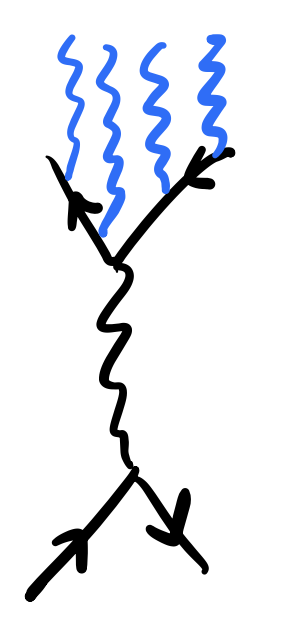
\includegraphics[scale=0.35]{Lectures/Images/lec14-multisoft.png}
\end{center}

We use the above scattering cross section as an example, but really, IR divergences are everywhere.

\begin{center}
    
\includegraphics[scale=0.35]{Lectures/Images/lec14-everywhere.jpg}
\end{center}

It is easy to see that there will be an IR issue in the diagram:

\begin{center}
    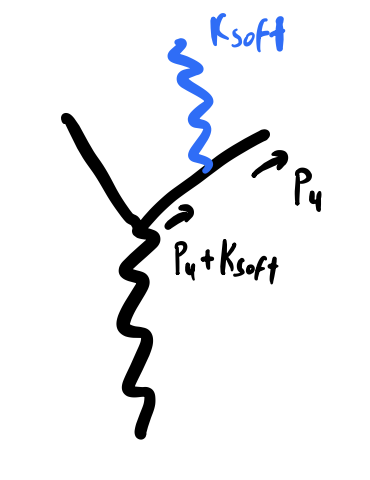
\includegraphics[scale=0.35]{Lectures/Images/lec14-softzoom.png}
\end{center}

Because this diagram contains the propagator:
\begin{equation}
    G_\psi(p_4 + k_{\text{soft}}) = \frac{-i(M + \slashed{p}_4 + \slashed{k}_{\text{soft}})}{(p_4 + k_{\text{soft}})^2 + M^2} \stackrel{p_4^2 = -M}{=} \frac{-i(\ldots)}{k_{\text{soft}}^2 + 2k_{\text{soft}} \cdot p_4} \sim \frac{1}{k_{\text{soft}} \cdot p_4}
\end{equation}
which diverges as $k_{\text{soft}} \to 0$.

\subsection{One-loop corrections at $e^-e^+ \to \mu^-\mu^+$}
What are the 1-loop corrections to $\mathcal{M}(e^-e^+ \to \mu^-\mu^+)$? We have the 6 diagrams (in addition to the single tree-level diagram we had previously):
\begin{center}
    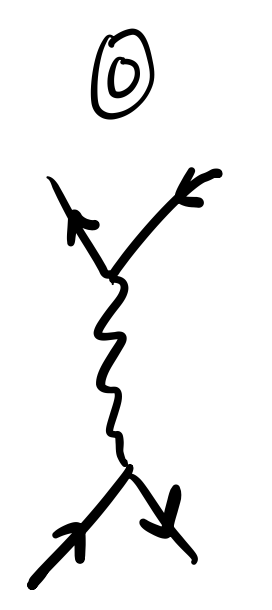
\includegraphics[scale=0.35]{Lectures/Images/lec14-treediagram.png}
\end{center}
\begin{center}
    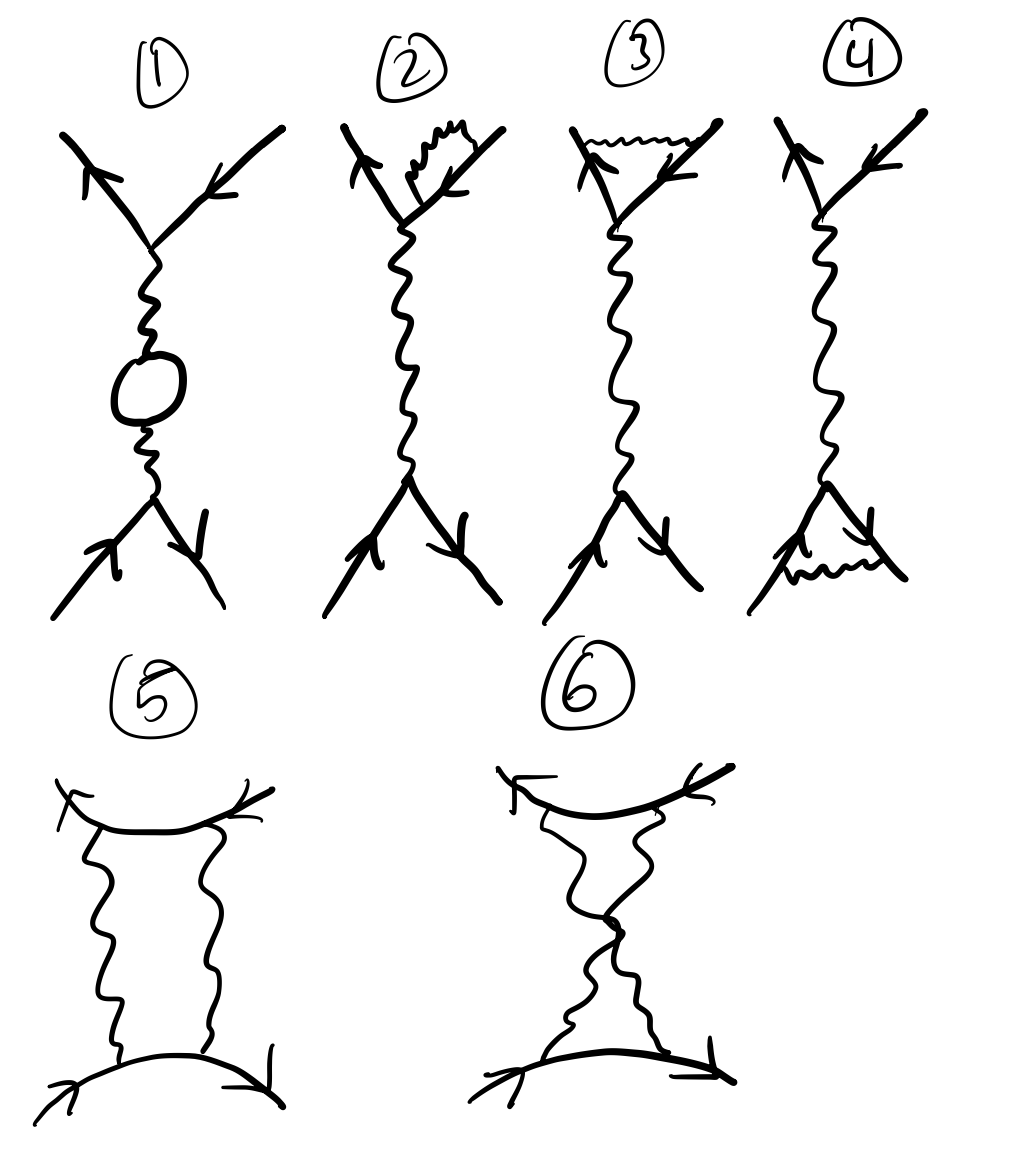
\includegraphics[scale=0.35]{Lectures/Images/lec14-oneloopdiagrams.png}
\end{center}

(2) drops out/does not contribute to the cross-section as the leg gets amputated. But this still looks pretty bad - 5 diagrams to calculate. But let's be a bit clever. Let's slightly modify QED and assign different charges $Q_e, Q_\mu \neq 1$ to the electron and muon. The reason to do this is:
\begin{equation}
    S_{\text{int}} = -e\int A_\nu(Q_e\bar{\psi}_e\gamma^\nu \psi_e + Q_\mu \bar{\psi}_\mu \gamma^\nu \psi_\mu)
\end{equation}
What is the motivation? Divergences in the electron and muon degrees of freedom have to cancel independently. Although we are interested in $Q_e = Q_\mu = 1$, this property nontheless carries over.

We start with looking at the effect the tree-level $\mathcal{M}_0$, which looking at diagram (0) we see $\mathcal{M}_0 \propto Q_eQ_\mu$ (each fermion vertex contributes a power of the respective charge). Let's look at the other diagrams. (1) is proportional to $Q_eQ_\mu Q_x^2$ because the fermion correction to the photon energy could come from any mystery fermion $x$ (it thus must cancel itself). (2) is not in $\mathcal{M}$. (3) is proportional to $Q_eQ_\mu^3$, (4) is proportional to $Q_e^3Q_\mu$, (5) is proportional to $Q_e^2Q_\mu^2$, and (6) is proportional to $Q_e^2Q_\mu^2$.

IR divergences proportional to any $Q_e^{c_e}Q_{\mu}^{c_\mu}$ have to cancel independently. We will focus on the $Q_eQ_\mu^3$ part/diagram (3) and look at its contribution to $\sigma \propto \abs{\mathcal{M}}^2$:

\begin{center}
    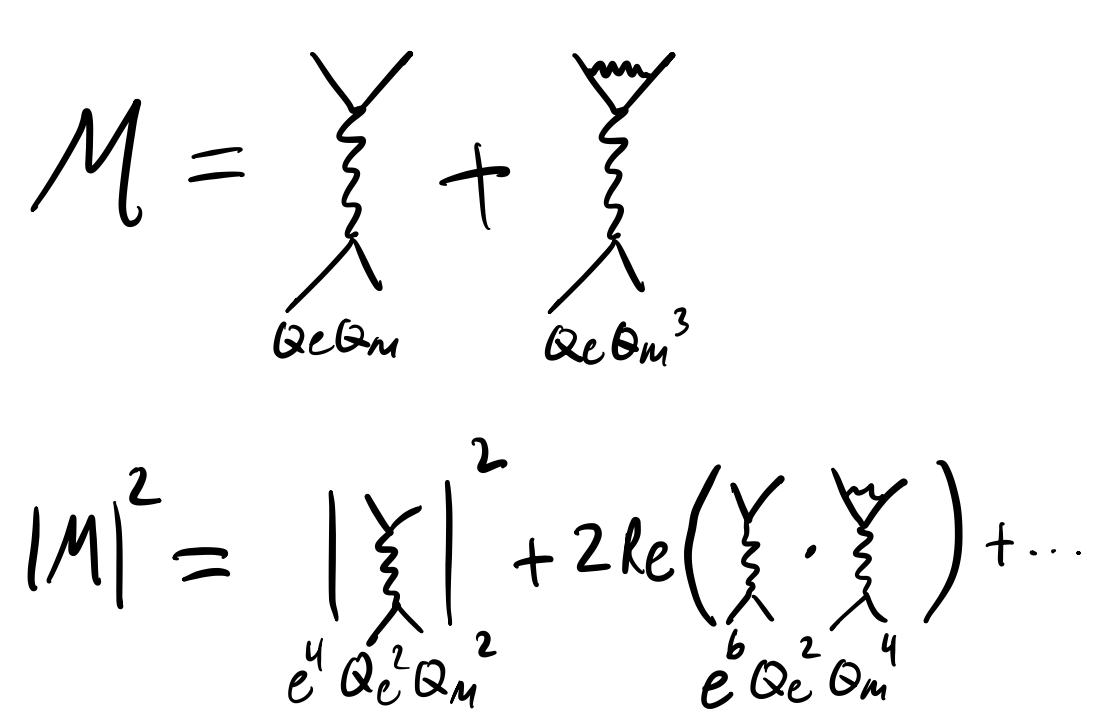
\includegraphics[scale=0.35]{Lectures/Images/lec14-oneloopcrosssection.png}
\end{center}

This correction indeed competes with the $\sigma(e^-e^+ \to \mu^-\mu^+\gamma)$ cross-section, because looking at the diagrams with the soft photon:

\begin{center}
    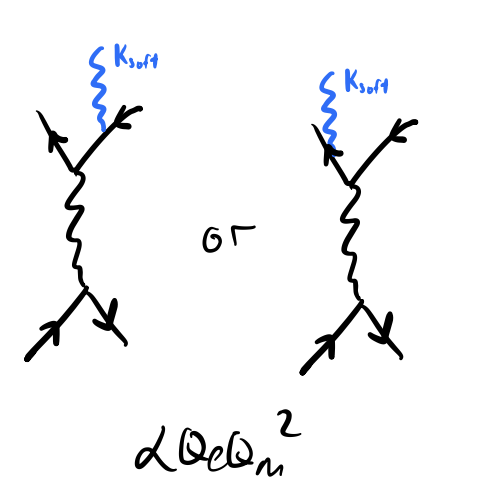
\includegraphics[scale=0.35]{Lectures/Images/lec14-softphotondiagrams.png}
\end{center}

(note that we can only put the soft photon on the muon leg) we see:
\begin{equation}
    \sigma(e^-e^+ \to \mu^-\mu^+\gamma) \sim \abs{\mathcal{M}}^2 \sim Q_e^2Q_\mu^4
\end{equation}

This trick with introducing fictitious charges is nice because it simplifies the analysis to specific diagrams. Let's now hone in and see how the divergences cancel.

\subsection{Computing the one-loop correction}
So, the only loop diagram we will have to consider is (3). The leading diagram is:

\begin{center}
    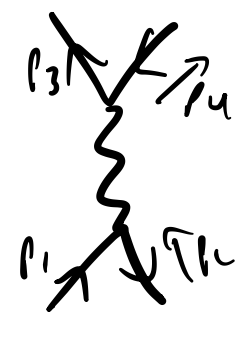
\includegraphics[scale=0.35]{Lectures/Images/lec14-treemomenta.png}
\end{center}

\begin{equation}
    i\mathcal{M}_0 = \frac{ie^2}{s}(\bar{v}_2\gamma^\rho u_1)(\bar{u}_3\gamma_\rho v_4)
\end{equation}

the 1-loop correction is:'

\begin{center}
    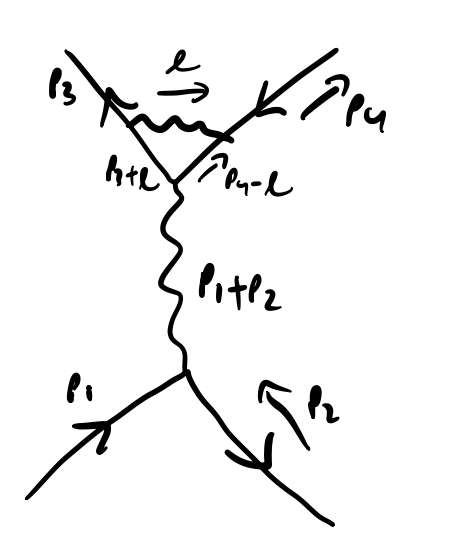
\includegraphics[scale=0.35]{Lectures/Images/lec14-oneloopmomenta.png}
\end{center}

\begin{equation}
    i\mathcal{M}_{\text{1-loop}} =  \frac{ie^2}{s}(\bar{v}_2\gamma^\rho u_1)(\bar{u}_3\Gamma_\rho v_4)
\end{equation}
with:
\begin{equation}
    \Gamma_\rho = \avg{j_\rho(p_1 + p_2)\psi\bar{\psi}(-p_4)}_{\text{amputated, 1-loop}}
\end{equation}

this is just an old friend! We will notice that this actually has IR divergences when we put the external legs on-shell, as is required by LSZ. Why didn't we notice? In RG we didn't put the external legs on shell, so we didn't see it. When we computed the electron dipole moment, we only looked at the terms which were IR safe. This is why many of the early calculations were successful, even though they didn't yet know how to handle these IR singularities.

Let's compute the diagram:

\begin{center}
    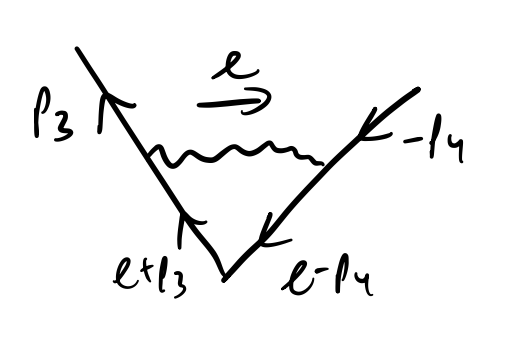
\includegraphics[scale=0.35]{Lectures/Images/lec14-oneloopmomentazoom.png}
\end{center}

We then have:
\begin{equation}
    \Gamma_\rho = \frac{(-ie)^2}{2}\avg{(\bar{\psi}\gamma^\rho\psi)_{p_1 + p_2}(\int A_\alpha \bar{\psi}\gamma^\alpha \psi)(\int A_\beta \bar{\psi}\gamma^\beta \psi)\psi \bar{\psi}(-p_4)}
\end{equation}
Wick contractions in order to get a connected diagram:

\begin{center}
    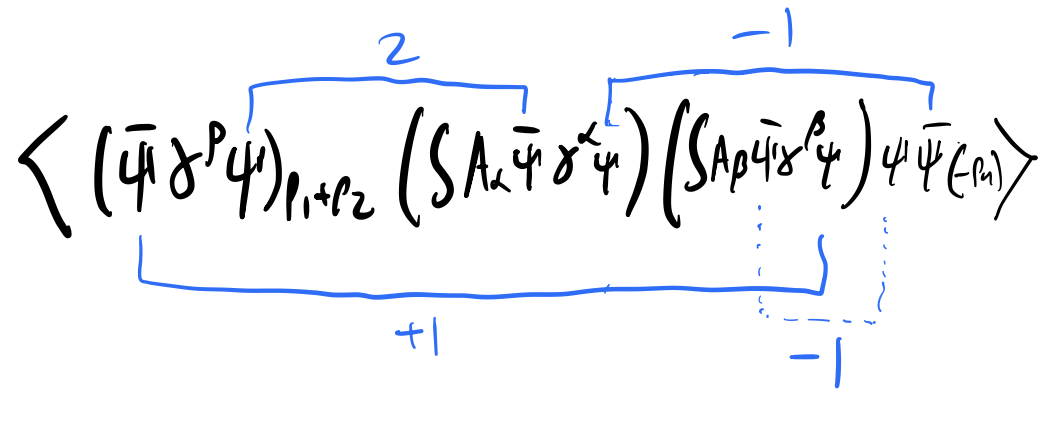
\includegraphics[scale=0.35]{Lectures/Images/lec14-pairings.png}
\end{center}

Thus:
\begin{equation}
    \Gamma_\rho = -e^2\int_l G(p_3)\gamma^\beta G(p_3 + l)\gamma^\rho G(l - p_4)\gamma^\alpha G(-p_4)G_{\alpha\beta}(l)
\end{equation}
If we amputate the external legs:
\begin{equation}
    \Gamma_\rho = -e^2\int_l \gamma^\beta G(p_3 + l)\gamma^\rho G(l - p_4)\gamma6\alpha G_{\alpha\beta}(l)
\end{equation}
Then we are left with (recalling that $G(p) = -\frac{-i}{M - \slashed{p}} = \frac{-i(M + \slashed{p})}{p^2 + M^2}$ and $G_{\alpha\beta}(l) = \frac{-i}{l^2}\eta_{\alpha\beta}$ choosing $\xi = 1$):
\begin{equation}
    \Gamma_\rho = -ie^2\int \frac{d^4l}{(2\pi)^4}\frac{\gamma_\alpha(M + \slashed{l} + \slashed{p}_3)\gamma^\rho (M + \slashed{l} - \slashed{p}_4)\gamma^\alpha}{l^2((l + p_3)^2 + M^2)((l - p_4)^2 + M^2)}
\end{equation}
so with $p_3^2 = p_4^2 = -M^2$ (on shell) the denominator becomes $l^2(l^2 + 2l\cdot p_3)(l^2 - 2l\cdot p_4)$ so as $l \to 0$ this goes as $l^2(l\cdot p_3)(l \cdot p_4)$ which implies:
\begin{equation}
    \Gamma_\rho \sim \frac{d^4l}{l^4}
\end{equation}
which is a (log) IR divergence. We can manifestly see how this arose from setting the momenta to be on-shell. This is actually a bit too quick. The above analysis looks like just a log divergence. But actually it can be even smaller, if $l$ is collinear with $p_{3/4}$ wherein the dot product vanishes. So when we integrate, we will see additional singularities arise from collinear momenta. This will lead to $\log^2$ singularities, which cannot be resummed via RG.

Before we show that this cancels with the other diagram, we need a way to compute it. In order to do this, we need to be able to regulate it. We will choose a simple but ugly IR regulator, i.e. giving the photon a mass $m_\gamma$. A more physical (but slighty harder to work with) regulator is to put things in a finite volume which gives the photon a maximum possible wavelength. In any case, with our choice of regulator the photon propagator transforms as:
\begin{equation}
    \frac{1}{l^2} \to \frac{1}{l^2 + m_\gamma^2}
\end{equation}
Focusing on the IR divergences, take $l \ll M, p_3, p_4$. For simplicity, we further assume high-energy scattering, i.e. $p_3, p_4 \gg M$. Then:
\begin{equation}
    \Gamma \cong ie^2\int_l \frac{\gamma_\alpha\slashed{p}_3\gamma^\rho \slashed{p}_4\gamma^\alpha}{(l^2 + m_\gamma^2)(l^2 + 2l \cdot p_3)(l^2 - 2l \cdot p_4)} = ie^2\int_l \frac{2\slashed{p}_4\gamma^\rho \slashed{p}_3}{(l^2 + m_\gamma^2)(l^2 + 2l \cdot p_3)(l^2 - 2l \cdot p_4)}
\end{equation}
If we sandwich the numerator with $\bar{u}_3 (\ldots)v_4$ then:
\begin{equation}
    \begin{split}
        \bar{u}_3 2\slashed{p}_4\gamma^\rho \slashed{p}_3v_4 &= 2\bar{u}_3\slashed{p}_4 \gamma^\rho \slashed{p}_3v_4 
        \\ &= -2\bar{u}_3(2p_3^\rho \slashed{p}_4 + \slashed{p}_4\slashed{p}_3 \gamma^\rho)v_4 
        \\ &= -2\bar{u}_3(2Mp_3^\rho - \slashed{p}_3\slashed{p}_4 \gamma^\rho - 2p_3 \cdot p_4 \gamma^\rho)v_4 
        \\ &= -2\bar{u}_3(2M(p_3^\rho - p_4^\rho) + M^2\gamma^\rho - 2p_3 \cdot p_4 \gamma^\rho)v_4 
        \\ &\stackrel{p_3, p_4 \gg M}{\approx} 4p_3 \cdot p_4 \bar{u}_3v_4 = -2s\bar{u}_3v_4
    \end{split}
\end{equation}
where in the last line we use:
\begin{equation}
    s = (-p_3 + p_4)^2 = 2M^2 - 2p_3 \cdot p_4 \approx -2p_3 \cdot p_4
\end{equation}
So at the end of the day, our $\Gamma_\rho$ looks like:
\begin{equation}
    \Gamma^\rho = -2ies\int \frac{d^4l}{(2\pi)^4}\frac{1}{(l^2 + m_\gamma^2)(l^2 + 2l \cdot p_3)(l^2 - 2l \cdot p_4)}
\end{equation}
So introducing Feynman parameeters with $x = l^2  +2l\cdot p_3$ and $y = l^2 - 2l \cdot p_4$ we have:
\begin{equation}
    \begin{split}
        \Gamma^\rho &= -4ies\int_0^1dx \int_0^{1-x}dy \int_l \frac{1}{[l^2 + 2l(p_3x - p_4y) + m_\gamma^2(1-x-y)]^3} 
        \\ &= -4ies\int_0^1dx \int_0^{1-x}dy \int_l \frac{1}{[(l + p_3x - p_4y)^2 + m_\gamma^2(1-x-y) - (p_3x - p_4y)^2]^3} 
        \\ &= -4ies\int_{xy}\int_q \frac{1}{(q^2 + \Delta)^3}
    \end{split}
\end{equation}
Which we can compute via Wick rotation:
\begin{equation}
    \stackrel{\text{Wick}}{\to} 4es \int_{xy}\frac{2\pi^2}{(2\pi)^4}\int_0^\infty \frac{dq q^3}{(q^2 + \Delta)^3}
\end{equation}
So then:
\begin{equation}
    \Gamma_\rho = \frac{es}{8\pi}\int_0^1 dx \int_0^{1-x}dy \frac{1}{\Delta}
\end{equation}
We will finish the calculation next week, but the $\Delta$ is $\sim m_\gamma^2 + xys$, the first integral gives $\sim \frac{\log(\ldots x)}{x}$ and the second gives $\log^2(\ldots)$, which is how the collinear singularities manifest, as we discussed. We will see that the result is $\sim \log(\frac{s}{m_\gamma})^2$.